
\section{System Design Details}

\subsection{Simulation Pipeline}

The general system workflow functions as Figure~\ref{fig:sim-pipeline}. System first initializes the environment based on the system setting config (e.g, see Table~\ref{tab:baseline_config}) or resumes from the previous experiment run. The specific initialization phases are shown in Table~\ref{tab:init_phases}.

Then the system enters into an execution cycle that allows agents to perceive and perform cognitive processing to plan for actions and update the environment accordingly. The execution phases are shown in Table~\ref{tab:execution_cycle}. Within this cycle, there is also a system validation and correction cycle over the agent's response and action to ensure its format and content are legal (see Figure~\ref{fig:retry-validation} and Table~\ref{tab:validation_layers}).

Please refer to those tables and figures for more details.

\begin{figure*}[htbp]
  \centering
  
\includegraphics[width=\textwidth]{figures/Sim-Pipline.drawio.pdf}
    \caption{\textbf{Simulation Pipeline Overview} showing the main components and data flow through the system architecture. The pipeline illustrates how the Singleton-based Checkpoint, modular microservices, and key simulation processes interact to maintain a consistent state and flow of information.}
  \label{fig:sim-pipeline}
  \end{figure*}
  


\begin{table*}[htbp]
  \centering
  \caption{Simulation Initialization Phases}
  \label{tab:init_phases}
  \small
  \setlength{\tabcolsep}{5pt}
  \begin{tabular}{p{3cm}p{10cm}}
    \toprule
    \textbf{Phase} & \textbf{Description} \\
    \midrule
    Configuration Loading \& Validation & 
    $\bullet$ Loads parameters from configuration file (prompt paths, agent types, rules, strategies) \newline
    $\bullet$ Validates type correctness, constraints, and completeness \newline
    $\bullet$ Creates authoritative configuration object for simulation \\
    \midrule
    Environment Setup & 
    $\bullet$ Plant Resources: \newline
    \quad - Generated based on configured abundance \newline
    \quad - Each plant gets a unique ID, initial quantity, capacity, nutrition value, and respawn delay \newline
    $\bullet$ Prey Animals: \newline
    \quad - Initialized with unique IDs \newline
    \quad - HP and max health sampled from a Gaussian distribution \newline
    \quad - Assigned physical ability values \newline
    $\bullet$ Resources placed randomly in unoccupied grid cells \\
    \midrule
    Initial Agent Spawning & 
    $\bullet$ Instantiates agents based on population size \newline
    $\bullet$ Assigns moral types according to configuration ratios \newline
    $\bullet$ Initializes attributes: HP, age, physical ability \newline
    $\bullet$ No initial family ties \\
    \midrule
    Execution Queue Setup & 
    $\bullet$ Creates randomized agent sequence for fair execution \newline
    $\bullet$ Initializes time step counter (typically 0 or 1) \newline
    $\bullet$ Sets up containers for agent observations \\
    \midrule
    Logging System Setup & 
    $\bullet$ Configures comprehensive tracking system \newline
    $\bullet$ Creates log files for: \newline
    \quad - Global progress summaries \newline
    \quad - Per-step execution records \newline
    \quad - Detailed event logs \newline
    \quad - Error diagnostics \newline
    $\bullet$ Organizes logs in uniquely named directories \\
    \bottomrule
  \end{tabular}
\end{table*}





\begin{table*}[htbp]
  \centering
  \caption{Per-Step Execution Cycle Phases}
  \label{tab:execution_cycle}
  \small
  \setlength{\tabcolsep}{5pt}
  \begin{tabular}{p{2.5cm}p{10cm}}
    \toprule
    \textbf{Phase} & \textbf{Description} \\
    \midrule
    Environment State Update & 
    $\bullet$ Updates plant lifecycle: restores depleted plants after respawn delay, increases quantity for non-depleted plants \newline
    $\bullet$ Spawns new prey in empty locations based on probability and maximum count \newline
    $\bullet$ Removes dead prey from the grid \\
    \midrule
    Agent Observation & 
    $\bullet$ Self-assessment: queries HP, age, inventory, physical ability, reproductive status \newline
    $\bullet$ Environmental perception: detects nearby resources, prey, and other agents \newline
    $\bullet$ Memory retrieval: accesses past observations, messages, and action outcomes \newline
    $\bullet$ Context formatting: structures information for LLM prompt \\
    \midrule
    Agent Decision Making & 
    $\bullet$ Constructs system message with agent persona and rules \newline
    $\bullet$ Builds user message with current state and context \newline
    $\bullet$ LLM processes context and returns proposed action \newline
    $\bullet$ Validates response format and structure \\
    \midrule
    Action Execution \& Validation & 
    $\bullet$ Performs response \& action validation \newline
    $\bullet$ Applies validated actions to simulation state \\
    \midrule
    State Finalization &
    $\bullet$ Updates agent HP, inventories, and environmental quantities \newline
    $\bullet$ Handles communication and memory updates \newline
    $\bullet$ Performs system-wide consistency checks \newline
    $\bullet$ Records detailed logs of agent states, environment state, and metrics \newline
    $\bullet$ Prepares state for next cycle \\
    \midrule
    Termination Check & 
    $\bullet$ Evaluates termination criteria (max steps, population collapse, goals) \newline
    $\bullet$ Either concludes simulation or increments time step \\
    \bottomrule
  \end{tabular}
\end{table*}





\begin{figure*}[htbp]
    \centering
    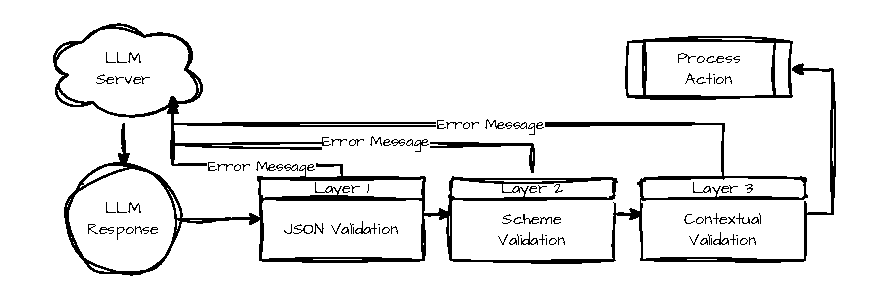
\includegraphics[width=0.9\textwidth]{figures/Retry-validation-layers.drawio.pdf}
    \caption{Multi-layer validation and retry framework showing the escalating levels of validation applied to agent actions. The diagram illustrates the three validation layers: syntactic and schema validation, contextual rule-based pre-validation, and action handler final validation, along with their respective feedback loops and retry mechanisms.}
    \label{fig:retry-validation}
\end{figure*}

\begin{table*}[htbp]
  \centering
  \caption{The Checklist of Multi-Layer Response \& Action Validation.}
  \label{tab:validation_layers}
  \small
  \setlength{\tabcolsep}{5pt}
  \begin{tabular}{p{2.5cm}p{10cm}}
    \toprule
    \textbf{Layer} & \textbf{Description} \\
    \midrule
    Layer 1: Syntactic and Schema & 
    $\bullet$ Applied immediately after LLM output generation \newline
    $\bullet$ Two critical checks: \newline
    \quad - Syntactic validation: Ensures proper JSON formatting \newline
    \quad - Schema validation: Verifies required fields, types, and enumerations \newline
    $\bullet$ Retry mechanism: \newline
    \quad - Resends prompt with error metadata \newline
    \quad - Limited to predefined maximum attempts \newline
    $\bullet$ Focus: Structural correctness only \\
    \midrule
    Layer 2: Contextual and Rule-Based & 
    $\bullet$ Domain-specific validation within Agent Decision Making phase \newline
    $\bullet$ Contextual checks: \newline
    \quad - Target existence and accessibility \newline
    \quad - Location-based constraints \newline
    \quad - HP sufficiency for action costs \newline
    $\bullet$ Memory constraints: \newline
    \quad - Long-term memory capacity limits \newline
    $\bullet$ Feedback loop: \newline
    \quad - Human-readable error messages \newline
    \quad - Updated prompts with feedback \newline
    \quad - Configurable retry rounds \\
    \midrule
    Layer 3: Action Handler Final & 
    $\bullet$ Executed during Action Execution phase \newline
    $\bullet$ Domain-specific validation in action handlers \newline
    $\bullet$ Dynamic condition checks: \newline
    \quad - Agent adjacency for physical interactions \newline
    \quad - HP sufficiency with current state \newline
    \quad - Race conditions with shared resources \newline
    $\bullet$ No LLM retry mechanism \newline
    $\bullet$ Failure handling: \newline
    \quad - Action nullification or failure processing \newline
    \quad - Logging to agent observation history \\
    \bottomrule
  \end{tabular}

\end{table*}






\subsection{System Design Principles}
The Morality-AI simulation is built on two core principles: centralized state management and modular architecture. A Singleton-based Checkpoint class maintains a single, authoritative simulation state, ensuring consistency, atomic updates, and easy reproducibility. This design prevents conflicting states and simplifies debugging and resuming experiments.
The system adopts a microservice-inspired structure, separating major functions—such as state persistence, agent reasoning, and LLM interfacing—into independent, easily testable modules. This modularity enhances maintainability, scalability, and flexibility, allowing components to be updated or replaced without affecting the overall system. Together, these principles provide a robust and extensible foundation for complex agent-based simulations.




\section{Agent Design Details}
\subsection{Agent Designs and Workflows}

Agents are the primary decision-making entities in the simulation. They possess a set of core attributes that govern their physical capabilities, cognitive constraints, and eligibility for specific actions (see the agent attributes in Table~\ref{tab:baseline_config}).


At the beginning of agent initialization, agent will be given their value/moral type prompt and all the system prompts like environment dynamics, requirement, commonsense strategies etc (prompt details see \ref{sec:prompts}). Then, during each execution cycle, the agent will be given the perception of the environment and its own status, and perform cognitive processing to make action plan. They will perform one round of reflection before finalize their response that contains their cognitive processing and action plan. The process follows Figure~\ref{fig:agent-decision} to make decisions.

For the current project, the structure of the agent's moral type is listed in Table~\ref{tab:moral_types}, with the rationale of the design choices in the main text. We want to note that these moral types is not the only way to define the value of an agent. The value can be defined in many other ways - one can focus on the action principles, or calculation of utility, or even be involved in culture and religion to study different problems.

The structure of the agent's perception space is listed in Table~\ref{tab:agent_perception}. The structure of the agent's cognition is listed in Table~\ref{tab:agent_cognition}. The content in the action space is listed in Table~\ref{tab:agent_actions}.




\begin{figure*}[htbp]
    \centering
    
\includegraphics[width=\textwidth,height=0.4\textheight,keepaspectratio,trim={2cm 16cm 2cm 2cm},clip]{figures/Agent-Decision-Process.drawio.pdf}
    \caption{The LLM query process for decision making, illustrating the flow from observation gathering through prompt construction, LLM interaction, and action validation. This process shows how environmental perceptions, agent state, and memory are integrated to produce contextually relevant decisions within the simulation environment.}
    \label{fig:agent-decision}
  \end{figure*}

  \begin{table*}[htbp]
    \centering
    \small
    \caption{Agent Moral Types Summary. Here, we summarize the core characteristics, expected typical behaviors, and expected cooperation patterns of these moral types. However, the simulated behavior for each agent might not strictly follow the expected behaviors due to the randomness of LLM's output. The exact prompt for each moral type is shown in \ref{sec:prompts}}
    \setlength{\tabcolsep}{4pt}
    \begin{tabular}{p{2cm}p{3.5cm}p{3.5cm}p{3.5cm}}
      \toprule
      \textbf{Moral Type} & \textbf{Core Characteristics} & \textbf{Expected Typical Behaviors} & \textbf{Expected Cooperation Pattern} \\
      \midrule
      Universal Group-Focused Moral & Aim for universal well-being and collective good, harm-action averse & Share resources freely; protect others from harm; communicate transparently & Highly altruistic and cooperative with all agents \\
      \midrule
      Reciprocal Group-Focused Moral & Fairness and mutual benefit within in-group, harm action allowed & Form strong bonds with cooperative peers & Cooperative with in-group; neutral or adversarial to out-group or selfish agents \\
      \midrule
      Kin-Focused Moral & Prioritize genetic relatives above all else, harm action allowed & Form close-knit kinship clusters; sacrifice for kin & Intensely altruistic toward family; indifferent or competitive toward non-kin \\
      \midrule
      Reproductive Selfish & Personal reproductive success, harm action allowed & Acquire resources for own survival; opportunistic tactics & Cooperate only when serving reproductive interests; inclined to hoard resources \\
      \bottomrule
    \end{tabular}
    \label{tab:moral_types}
  \end{table*}

\begin{table*}[htbp]
    \centering
    \caption{Agent Cognition Structure (Memory, Judgement and Planning)}
    \label{tab:agent_cognition}
    \small
    \setlength{\tabcolsep}{4pt}
    \begin{tabular}{p{4cm}p{9cm}}
    \toprule
    \textbf{Field} & \textbf{Key Subfields / Description} \\
    \midrule
    \textbf{1. Prey-Based Cognition} &
    $\bullet$ Organized by prey\_id: \newline
    \hspace*{1em} $\circ$ hunt\_fact\_history\_of\_this\_prey: who hunted, effect, time step, damage, if\_killed \newline
    \hspace*{1em} $\circ$ communication\_and\_planning\_before\_killing\_prey: reward, collaborators, distribution plan, objections \newline
    \hspace*{1em} $\circ$ distribution\_after\_killing\_prey: winner, allocation, fairness evaluation, free rider check \newline
    \hspace*{1em} $\circ$ plan\_next: next plan, retaliation plan, stage, reasoning \newline
    \hspace*{1em} $\circ$ afterward\_happenings: retaliation events, other events, lessons learned \\
    \midrule
    \textbf{2. Agent-Based Cognition} &
    $\bullet$ Organized by agent\_id: \newline
    \hspace*{1em} $\circ$ important\_interaction\_history: what\_i\_did\_to\_him, what\_he\_did\_to\_me (action type, success, reason, target moral type) \newline
    \hspace*{1em} $\circ$ thinking: evaluation, judgement, relationship, agreement, plan \\
    \midrule
    \textbf{3. Family Plan} &
    $\bullet$ Organized by agent\_id: \newline
    \hspace*{1em} $\circ$ status: how the family member is doing \newline
    \hspace*{1em} $\circ$ plan: what to do to/with them \\
    \midrule
    \textbf{4. Reproduction Plan} &
    $\bullet$ thinking: reasoning about reproduction plan \newline
    $\bullet$ preconditions\_and\_subgoals: specific preconditions needed \newline
    $\bullet$ estimated\_time\_to\_produce\_next\_child: time step \\
    \midrule
    \textbf{5. Learned Strategies} &
    $\bullet$ Lessons learned, strategies to follow in the future \\
    \bottomrule
    \end{tabular}
\end{table*}

\begin{table*}[htbp]
    \centering
    \caption{Agent Perception Content Structure}
    \label{tab:agent_perception}
    \small
    \setlength{\tabcolsep}{4pt}
    \begin{tabular}{p{4cm}p{9cm}}
    \toprule
    \textbf{Category} & \textbf{Description} \\
    \midrule
    Self/Internal Information & 
    $\bullet$ Current HP and health status \newline
    $\bullet$ Family relationships and status \newline
    $\bullet$ Personal attributes and capabilities \\
    \midrule
    Environment Status & 
    $\bullet$ Available plant resources \newline
    $\bullet$ Prey animals present in the environment \newline
    $\bullet$ Resource locations and quantities \\
    \midrule
    Other Agents Status & 
    $\bullet$ Basic information (age, HP) of other agents \newline
    $\bullet$ Moral types of other agents \newline
    $\bullet$ Current positions and states \\
    \midrule
    Recent History & 
    $\bullet$ Last 15 steps of personal interactions: \newline
    \hspace*{1em} - Others' actions and communications toward self \newline
    \hspace*{1em} - Self's actions toward environment and others \newline
    $\bullet$ Recent events: \newline
    \hspace*{1em} - Changes in environment and other agents \newline
    \hspace*{1em} - Family-related news and updates \newline
    $\bullet$ Hunting activities: \newline
    \hspace*{1em} - Personal involvement in prey hunting \newline
    \hspace*{1em} - Related communications and outcomes \\
    \midrule
    Memory & 
    $\bullet$ Updated memory from previous step \newline
    $\bullet$ Immediate action plans from previous step \\
    \bottomrule
    \end{tabular}
\end{table*}


  


\begin{table*}[htbp]
  \centering
  \caption{Agent Action Space Summary}
  \label{tab:agent_actions}
  \small
  \setlength{\tabcolsep}{4pt}
  \begin{tabular}{p{1.5cm}p{3cm}p{3cm}p{2cm}p{3cm}}
  \toprule
    \textbf{Action} & \textbf{Description} & \textbf{Requirements} & \textbf{HP Cost} & \textbf{Outcome} \\
    \midrule
    \multicolumn{5}{l}{\textit{(Re)Production Actions}} \\
    \midrule
    Collect & Gather plant resources from environment & Resource exists and is a plant node & None & Agent gains HP (quantity $\times$ nutrition value); plant quantity reduced \\
    \midrule
    Hunt & Target prey animals for nutritional gain & Prey exists & 1 HP + additional damage if failed & If successful, prey killed and agent receives reward equal to prey's max HP \\
    \midrule
    Reproduce & Create offspring & Minimum age and HP thresholds met & Defined in reproduction parameters & Child agent created with age 0 and initial HP, inheriting parent's archetype \\
    \midrule
    \multicolumn{5}{l}{\textit{Social Interaction Actions}} \\
    \midrule
    Allocate & Transfer HP to other agents & Targets exist and are alive; sufficient HP & Equal to HP transferred & Recipients gain specified HP (capped at maximum) \\
  \midrule
    Fight & Attempt to damage another agent & Target exists, is alive, not self & 1 HP resistance cost & If successful (based on ability difference), target suffers damage equal to attacker's ability \\
  \midrule
    Rob & Forcibly transfer HP from another agent & Target exists and is alive & 1 HP + potential failure penalty & If successful, HP transferred from target to robber \\
  \midrule
    Communicate & Send messages to other agents & Target agents exist and are alive & None & Message recorded in recipient's memory \\
  \midrule
    \multicolumn{5}{l}{\textit{Other Actions}} \\
  \midrule
    DoNothing & Abstain from all actions & None & None & No changes to agent or environment \\
  \bottomrule
  \end{tabular}
  \end{table*}
  


\subsection{The Quantitative Model for Calculating Action Results}

The success rate and damage point in actions like hunting, robbery, etc, is calculated based on the physical ability of the agents. The physical ability values are initialized as a random number from a Gaussian distribution with specified mean and standard deviation in the configuration file Table~\ref{tab:baseline_config} (with 0 standard deviation, there will be no random variation). Note that prey also has a physical ability value that is initialized in the same way. 

\paragraph{Success Rate}
The success of hunt, fight, and rob actions takes on probabilistic manner. The success of such actions depends on the relative physical abilities of the involved entities. Let $\Delta \mathrm{PA} = \mathrm{PA}_k - \mathrm{PA}_{target}$ represent the physical ability differential between an actor $k$ and a target entity (which could be another agent $j$ or a prey animal $A_j$). The probability of success, $P_{succ}$, for these actions is determined by the function:
% $$ P_{succ}(\Delta \mathrm{PA}; I_{\mathrm{PA},k}, S_{\mathrm{PA},k}) = \min\left(\max\left((0.5 + I_{\mathrm{PA},k}) + 0.4 \cdot \tanh\left(\frac{\Delta \mathrm{PA}}{S_{\mathrm{PA},k}}\right), 0.1\right), 0.9\right) $$
\begin{align*}
&P_{succ}(\Delta \mathrm{PA}; I_{\mathrm{PA},k}, S_{\mathrm{PA},k}) = \min\\&\left(\max\left((0.5 + I_{\mathrm{PA},k}) + 0.4 \cdot \tanh\left(\frac{\Delta \mathrm{PA}}{S_{\mathrm{PA},k}}\right), 0.1\right), 0.9\right)
\end{align*}
Here, $I_{\mathrm{PA},k}$ and $S_{\mathrm{PA},k}$ are agent $k$'s specific scaling parameters (an intercept offset and a slope divisor, respectively) pertinent to physical ability interactions, derived from its configuration. The function $\min(\max(x,a),b)$ ensures the probability is clipped to the interval $[a,b]$, in this case, $[0.1, 0.9]$. The outcome of such an action is then determined by a Bernoulli trial $X \sim \text{Bernoulli}(P_{succ})$.

In the descriptions that follow, $\HP_k(t')$ signifies the health of agent $k$ after any initial action-specific costs have been deducted, but before other consequences of the action (e.g., gains from success, damage from failure) are applied.

\paragraph{Collect}
Agent $k$ may attempt to gather resources from a designated plant node $P_i$, which possesses a current resource quantity $Q_i(t)$. The agent specifies a desired quantity $q_{req}$. For the action to be valid, $P_i$ must be a plant, and its available quantity must meet the request, i.e., $Q_i(t) \ge q_{req}$. The actual quantity gathered, $q_{coll}$, is constrained by the request, availability, and the agent's single-action collection capacity, $k_{collect}$ (a global limit):
$$ q_{coll} = \min(q_{req}, Q_i(t), k_{collect}) $$
A positive quantity must be collectible ($q_{coll} > 0$). Consequently, the agent's health and the plant's resources are updated as follows:
\begin{align*}
    &\HP_k(t+1) = \\
    &\bound{\HP_k(t) + q_{coll} \cdot H_{plant}}{0}{\HP_{k,max}} \\
    & Q_i(t+1) = Q_i(t) - q_{coll}
\end{align*}
where $H_{plant}$ denotes the nutritional value conferred per unit of the plant resource. This action imparts no direct HP cost to agent $k$.

\paragraph{Allocate}
An agent $k$ (the donor) can transfer Health Points to other agents. This is specified via an \texttt{allocation\_plan}, $(h_{kj})_{j \in J}$, where $h_{kj} \in \mathbb{R}^+$ is the amount of HP designated for transfer to each target agent $j$ in a non-empty set $J \subset \mathcal{K}(t)$. The total HP intended for allocation by agent $k$ is $H_{alloc,k} = \sum_{j \in J} h_{kj}$. This action is permissible if all target agents $j \in J$ are alive and the donor possesses sufficient HP, specifically $\HP_k(t) > H_{alloc,k}$. If valid, the HP of the involved agents is then adjusted:
\begin{align*}
    &\forall j \in J,\\ \quad &\HP_j(t+1) = \bound{\HP_j(t) + h_{kj}}{0}{\HP_{j,max}} \\
    &\HP_k(t+1) = \\
    &\bound{\HP_k(t) - H_{alloc,k}}{0}{\HP_{k,max}}
\end{align*}

\paragraph{Fight}
Agent $k$ (attacker) may engage agent $j$ (target), provided $k \neq j$ and $j$ is alive. To initiate a fight, the attacker $k$ incurs an immediate cost $C_{fight,init} = 1$ HP:
$$ \HP_k(t') = \HP_k(t) - C_{fight,init} $$
If $\HP_k(t') \le 0$, agent $k$ is removed from $\mathcal{K}(t+1)$. Otherwise, the outcome of the fight is determined by a Bernoulli random variable $X_{fight} \sim \text{Bernoulli}(P_{succ}(\Delta \mathrm{PA}_{kj}; I_{\mathrm{PA},k}, S_{\mathrm{PA},k}))$, where $\Delta \mathrm{PA}_{kj} = \mathrm{PA}_k - \mathrm{PA}_j$. The health point dynamics for both the target and attacker, contingent on the outcome $X_{fight}$, are:
\begin{itemize}
    \item If $X_{fight}=1$ (success): The target's health is reduced, $\HP_j(t+1) = \bound{\HP_j(t) - \lfloor \mathrm{PA}_k \rfloor}{0}{\HP_{j,max}}$.
    \item If $X_{fight}=0$ (failure): The target's health remains unchanged, $\HP_j(t+1) = \HP_j(t)$.
\end{itemize}
In both scenarios, the attacker's health after the interaction resolves is $\HP_k(t+1) = \HP_k(t')$. The target agent $j$ is removed if its health $\HP_j(t+1) \le 0$.

\paragraph{Rob}
Agent $k$ (robber) may attempt to forcibly extract $h_{rob,req} > 0$ HP from a target agent $j$, provided $j$ is alive and possesses sufficient health ($\HP_j(t) \ge h_{rob,req}$). The robber $k$ first incurs an initiation cost $C_{rob,init} = 1$ HP:
$$ \HP_k(t') = \HP_k(t) - C_{rob,init} $$
If $\HP_k(t') \le 0$, $k$ is removed. Otherwise, the success of the attempt is a random variable $X_{rob} \sim \text{Bernoulli}(P_{succ}(\Delta \mathrm{PA}_{kj}; I_{\mathrm{PA},k}, S_{\mathrm{PA},k}))$, with $\Delta \mathrm{PA}_{kj} = \mathrm{PA}_k - \mathrm{PA}_j$. Depending on the outcome $X_{rob}$, the HP updates are:
\begin{itemize}
    \item If $X_{rob}=1$ (success):
    \begin{align*}
        \HP_j&(t+1) = \\&\bound{\HP_j(t) - h_{rob,req}}{0}{\HP_{j,max}} \\
        \HP_k&(t+1) = \\&\bound{\HP_k(t') + h_{rob,req}}{0}{\HP_{k,max}}
    \end{align*}
    The target $j$ is removed if $\HP_j(t+1) \le 0$.
    \item If $X_{rob}=0$ (failure): No HP is transferred, thus $\HP_j(t+1) = \HP_j(t)$, and the robber's health remains $\HP_k(t+1) = \HP_k(t')$.
\end{itemize}

\paragraph{Hunt}
Agent $k$ (hunter) may target a prey animal $A_j$, characterized by physical ability $\mathrm{PA}_{A_j}$ and health $\HP_{A_j}(t)$ (with maximum $\HP_{A_j,max}$). The hunter $k$ incurs an initial cost $R_{hunt}=1$ HP:
$$ \HP_k(t') = \HP_k(t) - R_{hunt} $$
If $\HP_k(t') \le 0$, $k$ is removed. Otherwise, the outcome is governed by $X_{hunt} \sim \text{Bernoulli}(P_{succ}(\Delta \mathrm{PA}_{kA_j}; I_{\mathrm{PA},k}, S_{\mathrm{PA},k}))$, where $\Delta \mathrm{PA}_{kA_j} = \mathrm{PA}_k - \mathrm{PA}_{A_j}$.
\begin{itemize}
    \item If $X_{hunt}=1$ (success): The prey $A_j$ sustains damage $D_{A_j} = \lfloor \mathrm{PA}_k \rfloor$, leading to $\HP_{A_j}(t+1) = \max(0, \HP_{A_j}(t) - D_{A_j})$.
        If this damage proves lethal ($\HP_{A_j}(t+1) \le 0$), prey $A_j$ is removed, and the hunter $k$ gains HP from the kill: 
        \begin{align*}
        &\HP_k(t+1) = \\&\bound{\HP_k(t') + \HP_{A_j,max}}{0}{\HP_{k,max}}
        \end{align*}
        If the prey survives the damage, the hunter gains no HP from the hit, so $\HP_k(t+1) = \HP_k(t')$.
    \item If $X_{hunt}=0$ (failure): The prey $A_j$ counter-attacks, inflicting $D_{prey}$ damage upon hunter $k$. This $D_{prey}$ is a characteristic of the prey (e.g., its counter-attack strength). The hunter's health is updated to 
        \begin{align*}
        &\HP_k(t+1) = \\&\bound{\HP_k(t') - D_{prey}}{0}{\HP_{k,max}}
        \end{align*}
        Hunter $k$ is removed if $\HP_k(t+1) \le 0$.
\end{itemize}

\paragraph{Reproduce}
An agent $k$ may create offspring if it meets age and health criteria: $Age_k(t) \ge Age_{repro,min}$ and $\HP_k(t) \ge \HP_{repro,min}$. Upon successful reproduction, a new agent $c$ is added to the population $\mathcal{K}(t+1)$, initialized with $Age_c(0)=0$ and health $\HP_c(0) = \HP_{child,init}$. The parent $k$ incurs an HP cost, $\HP_{repro,cost}$, resulting in an updated health:
\begin{align*}
    &\HP_k(t+1) = \\&\bound{\HP_k(t) - \HP_{repro,cost}}{0}{\HP_{k,max}}
\end{align*}

\paragraph{Communicate}
Agent $k$ can send a textual message $M$, constrained by length ($|M| \le L_{msg,max}$), to a specified set of recipient agents $J \subset \mathcal{K}(t)$. All recipients must be alive. This action does not directly alter HP.

\paragraph{DoNothing}
An agent $k$ may elect to perform no explicit action. This choice has no effect on its state or the environment; thus, $\HP_k(t+1) = \HP_k(t)$.
